\section{Surface Density of VH$z$Qs}
One interesting question to ask is given the compilation of VH$z$Qs
assembled here, are there bright $z>5.00$ quasars that are in {\it
current} photometric datasets, and if so, how many are still to be
discovered and confirmed spectroscopically?

In the North, we assume the UHS J-band depth of 19.6 \citep[Vega;
][]{Dye2018}.  In the South, one can use the report {\tt ABmagLimits}
for each survey in the database, we can calculate the depths of the
various NIR VISTA surveys.  Fig.~\ref{fig:VHS_J_abMagLim} shows this
calculated average {\tt AB MAGLIM} in the VHS.  As one can see, the
VHS is not completely uniform. The area wrapping round
310$\lesssim$RA/deg$\lesssim$90 and -70$\lesssim$ Decl./ deg
$\lesssim$ -40 has a $J$-band depth of 21.2 AB mag, whereas the rest
of the VHS area, the $J$-band depth is closer to 20.6 AB mag.

\begin{figure}
  \centering
  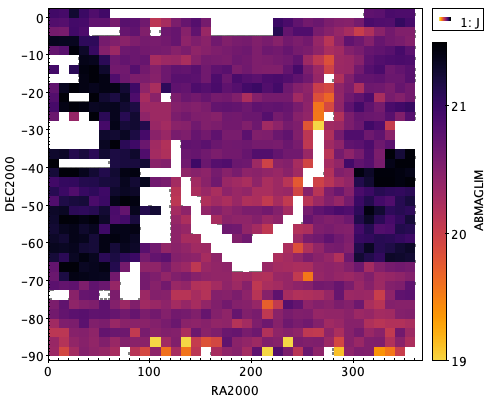
\includegraphics[width=8.5cm]{../data/WSA_VSA/VHS_J_abMagLim.png}
  \caption{The calculated average {\tt AB MAGLIM} in the VHS.
    As one can see, VHS is not completely uniform. The are 3 areas with different filter sets, 
    and the depths changed in 2 of these areas, particularly in $J$ and $K_{s}$. 
    Y and H are almost uniform, but the coverage is much less.}
  \label{fig:VHS_J_abMagLim}
\end{figure}

Having obtained an as-near-to-homogenous set of photometry as we can, 
we are now in a position to calculate the Absolute Magnitudes of the VH$z$Q 
sample and in particulare the absolute magnitude at rest-frame 1450\AA\ , $M_{1450}$, 
which is a key physical quantity and goes directly towards the quasar luminosity 
function and thus the reionization of hydrogen calculation. 

We calculate the Distance Modulus in the normal fashion, 
\begin{equation}
m_{1450} - M_{1450} = 5 \log \left (    \frac{ D_{\rm L}(z)}{\rm Mpc}  \right )  + 25 + K_{\rm corr}(X,z)
\end{equation}
where $m_{1450}$ is the apparent magnitude at 1450\AA\ ,  
%$M_{1450}$ is the absolute magnitude at 1450 \AA\ , 
$D_{\rm L}(z)$ is the luminosity distance and 
$K_{\rm corr}(X,z)$ is the $K$-correction which corrects for the effects of redshifting of the bandpass and the spectrum. 

The $m_{1450}$ apparent magnitude is derived from the $z-$, $y/Y-$ or $J-$band photometery.
%%
The Pan-STARSS1 $z_{\rm PS1}$ and $y_{\rm PS1}$-bands approximatley
sample the redshift ranges $4.53\leq z \leq 5.45$ and $5.28\leq z \leq 6.47$, respectively 
for 1450\AA'\ emission, while the VIRCAM $Y_{\rm VIRCAM}-$ and $J_{\rm VIRCAM}$-bands 
cover $5.50\leq z \leq 6.57$ and $7.06\leq z \leq 8.16$. 

\citet{Ross2013} has a detailed discussion of the $K$-correction (see that papers' Appendix B). 
The key result in that paper is, if quasars are described as having a power-law slope, 
$\alpha^{\nu}$ in spectral flux density, i.e., $f_\nu(\nu) \propto \nu^{\alpha_{\nu}}$ (as is conventional) 
then 
\begin{equation}
K_{\rm corr}(z) = -2.5 (1 + \alpha_{\nu}) \log[1 + z].
\end{equation}
Here the $[-2.5 \log(1 + z)]$ term corrects for the effective narrowing of the filter width with redshift, (the ``bandpass correction'') and the $[-2.5 \alpha^{\nu} \log(1 + z)]$ term takes into account the spectral index correction. The bandpass correction is approximately $\approx -1.945$ at redshift $z=5$ decreasing to $-2.32$ at redshift $z=7.50$. 

%At $z=5.00$, the rest-frame 1450\AA\ emission is redshifted to 8700\AA\ observed, i.e., in the $z$-band, while at $z=6.00$, $z=5.00$

\iffalse
\begin{figure*}
  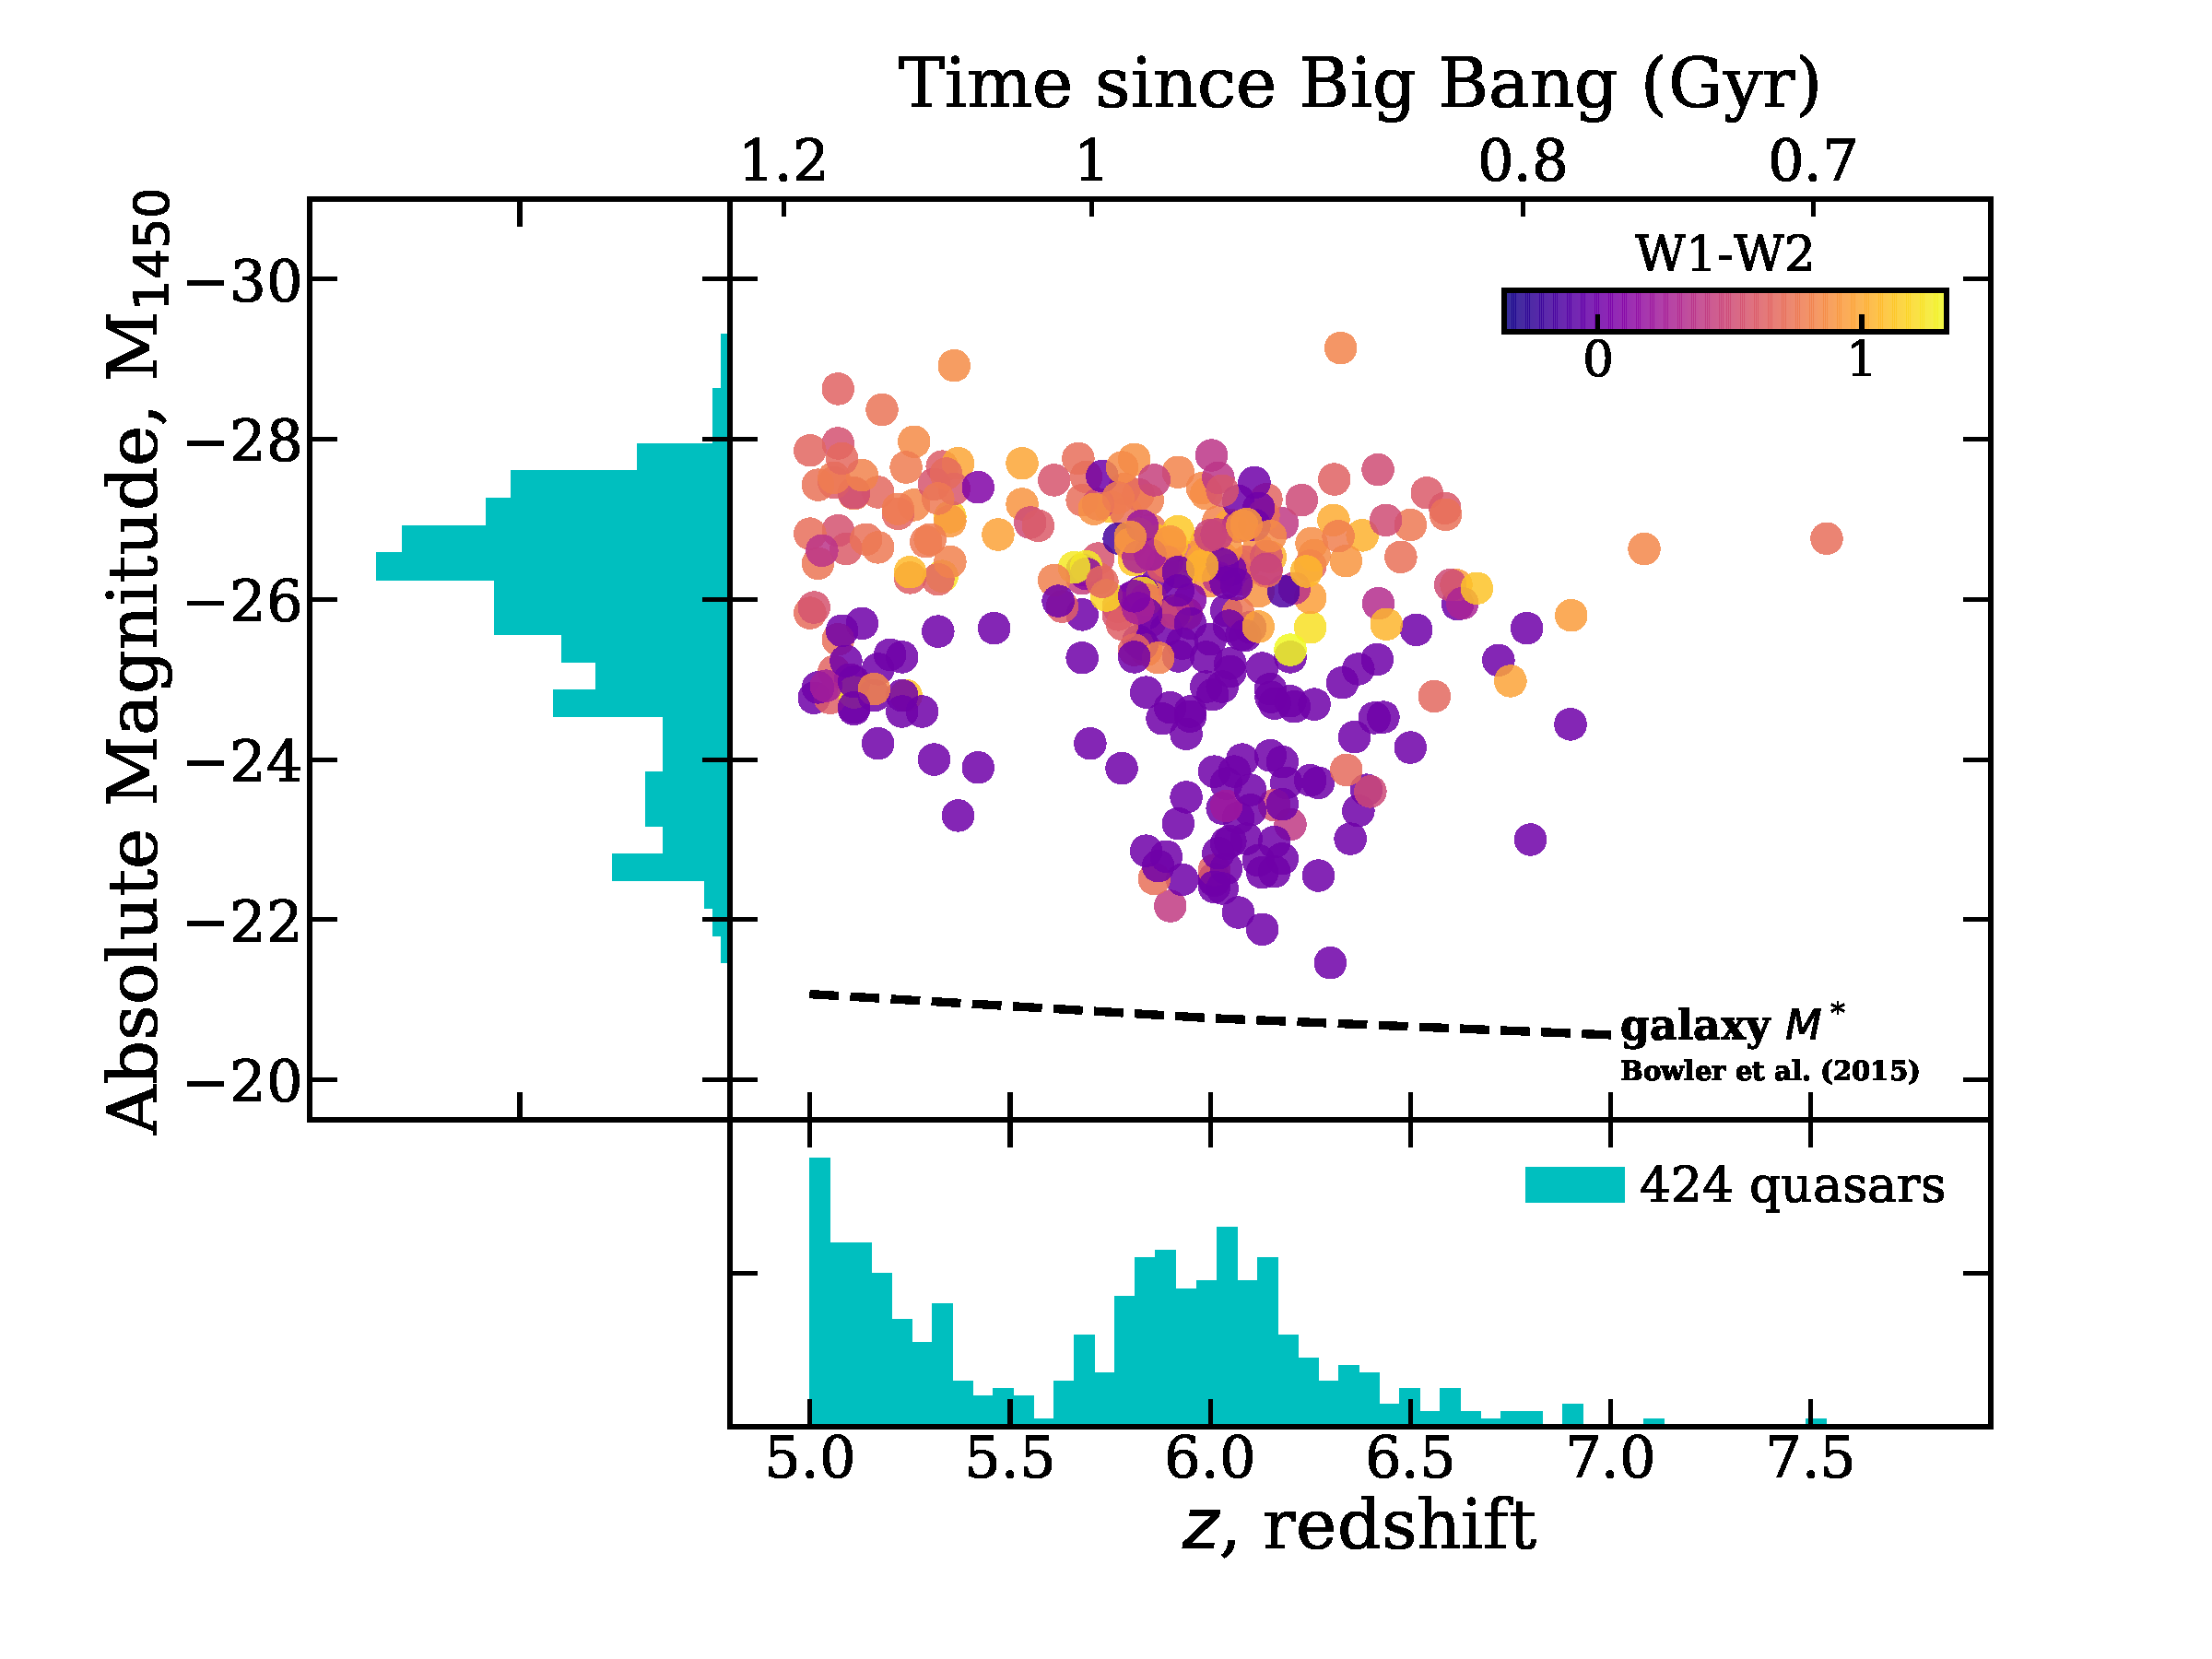
\includegraphics[width=18.0cm]
  {/cos_pc19a_npr/programs/quasars/highest_z/Lz/VHzQ_Lz_20180702.pdf}
  \centering
  \caption[]{The luminosity-redshift, $L-z$, plane for the VH$z$Qs. 
    The evolution of $M^{\star}$, the characteristic magnitude 
    for $z\simeq4–8$ galaxies is given by the long dashed line \citep{Bowler2015}. }
  \label{fig:Lz}
\end{figure*}
\fi


Following \citet{Fan2001b} and \citet{McGreer2013}, we use use an
exponential decline to describe the space density of VH$z$Qs at high
redshifts, e.g.
\begin{equation}
\rho(z, {\rm M}_{1450}) \propto 10^{k (z)}
\end{equation}
where $z$ is the sample redshift. 
